% fs-08-OneSample.tex

\documentclass[xcolor=dvipsnames]{beamer}
\usepackage{teachbeamer}

\title{One Sample}
\subtitle{{\CourseNumber}, BCIT}

\author{\CourseName}

\date{March 8, 2017}

% \begin{figure}[h]
% 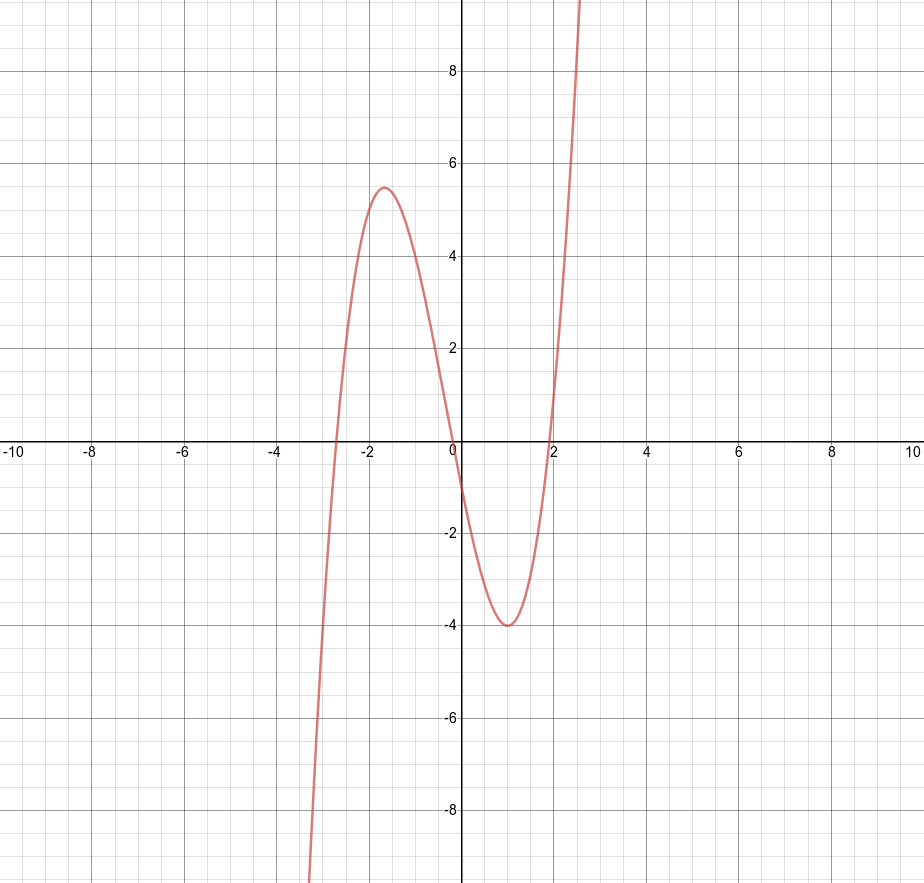
\includegraphics[scale=.3]{./diagrams/extrema1.png}
% \end{figure}

% Command             10pt    11pt    12pt
% \tiny               5       6       6
% \scriptsize         7       8       8
% \footnotesize       8       9       10
% \small              9       10      10.95
% \normalsize         10      10.95   12

\begin{document}

\begin{frame}
  \titlepage
\end{frame}

\begin{frame}
  \frametitle{Estimating a Population Proportion}
When you take a sample, you can try to estimate population parameters
such as mean, variance, and proportion on the basis of your sample
data. Let's think about population proportions first.
\begin{description}
\item[point estimate] The sample proportion (denoted by $\hat{p}$) is
  the best point estimate of the population proportion $p$.
\item[confidence interval] We can use a sample proportion to construct
  a confidence interval for the true value of a population proportion.
\item[sample size] We can find the sample size necessary to estimate a
  population proportion to a given degree of accuracy.
\end{description}
A \alert{point estimate} is a single value (or point) used to
approximate a population parameter.
\end{frame}

\begin{frame}
  \frametitle{Estimating a Population Proportion}
\beispiel{Yoghurt Expiry} You test 243 yoghurts three days after their
expiry date and find that 19 of them are spoiled. Find the best point
estimate of the percentage of this kind of yoghurt that spoils by day
three after the expiry date. Answer: the best point estimate is
$19/243$ or approximately $7.82$\%.

\bigskip

\begin{description}
\item[confidence interval] A confidence interval is a range of values
  used to estimate the true value of a population parameter. 
\item[confidence level] The confidence level is the probability
  $1-\alpha$ (such as 0.95 or 95\%) that the confidence interval
  actually contains the population parameter. The confidence level is
  also called the degree of confidence or the confidence coefficent.
\end{description}
\end{frame}

\begin{frame}
  \frametitle{Estimating a Population Proportion}
\begin{figure}[h]
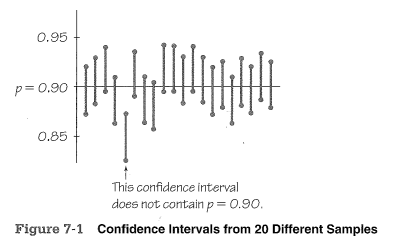
\includegraphics[scale=1]{./diagrams/triola-321.png}
\end{figure}
\end{frame}

\begin{frame}
  \frametitle{Estimating a Population Proportion}
\begin{figure}[h]
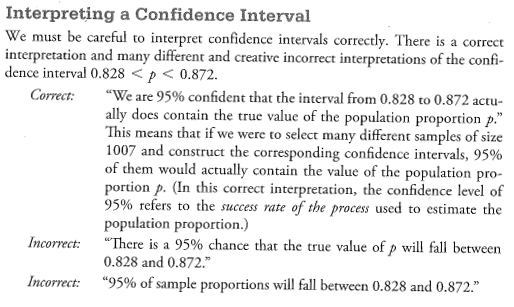
\includegraphics[scale=.8]{./diagrams/triola-320.png}
\end{figure}
\end{frame}

\begin{frame}
  \frametitle{Estimating a Population Proportion}
  \begin{description}
  \item[critical value] A critical value is the number on the
    borderline separating sample statistics that are likely to occur
    from those that are unlikely. The number $z_{\alpha/2}$ is a
    critical value that is a $z$-score with the property that it
    separates an area of $\alpha/2$ in the right tail of the standard
    normal distribution.
  \item[margin of error] When data from a simple random sample are
    used to estimate a population proportion $p$, the margin of error,
    denoted by $E$, is the maximum likely difference (with probability
    $1-\alpha$, such as 0.95) between the observed sample probability
    $\hat{p}$ and the true value of the population proportion $p$.
  \end{description}
\end{frame}

\begin{frame}
  \frametitle{Estimating a Population Proportion}
\begin{figure}[h]
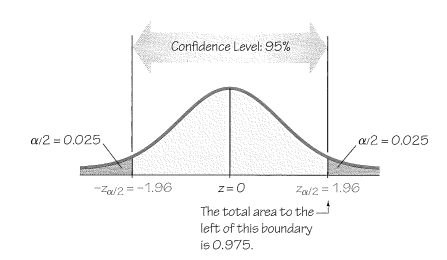
\includegraphics[scale=1]{./diagrams/triola-323a.png}
\end{figure}
\end{frame}

\begin{frame}
  \frametitle{Estimating a Population Proportion}
\begin{figure}[h]
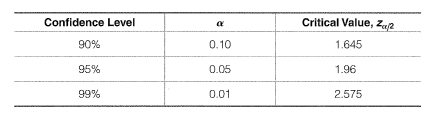
\includegraphics[scale=1]{./diagrams/triola-323b.png}
\end{figure}
\end{frame}

\begin{frame}
  \frametitle{Estimating a Population Proportion}
  \begin{block}{Formula for Margin of Error}
    \begin{equation}
      \label{eq:fidahyei}
      E=z_{\alpha/2}\sqrt{\frac{\hat{p}\hat{q}}{n}}
    \end{equation}
  \end{block}

\bigskip

The \alert{confidence interval} is $\hat{p}-E<p<\hat{p}+E$.
\end{frame}

\begin{frame}
  \frametitle{Sample Size to Estimate a Population Proportion}
  \begin{description}
  \item[Objective] Determine how large the sample $n$ should be in
    order to estimate the population proportion $p$
  \item[Notation] $p$ is the population proportion; $\hat{p}$ is the
    sample proportion; $n$ is the number of sample values; $E$ is the
    desired margin of error; and $z_{\alpha/2}$ is the $z$-score
    separating an area of $\alpha/2$ in the right tail of the standard
    normal distribution
  \item[Required] The sample must be a simple random sample of
    independent sample units
  \end{description}
\end{frame}

% \begin{frame}
% \begin{tabular}{|l|c|}\hline
% \hspace{1in} & \hspace{1in} \\
%   When an estimate $\hat{p}$ is known & $\displaystyle n=\frac{\left(z_{\alpha/2}\right)^{2}\hat{p}\hat{q}}{E^{2}}$ \\
% \hspace{1in} & \hspace{1in} \\ \hline
% \hspace{1in} & \hspace{1in} \\ 
%   When no estimate $\hat{p}$ is known & $\displaystyle n=\frac{\left(z_{\alpha/2}\right)^{2}\cdot{}0.25}{E^{2}}$ \\
% \hspace{1in} & \hspace{1in} \\ \hline
% \end{tabular}

% \bigskip

% If the computed sample size $n$ is not a whole number, round the value
% of $n$ \alert{up} to the next larger whole number.
% \end{frame}

\begin{frame}
  \frametitle{Sample Size to Estimate a Population Proportion}
  \begin{block}{estimate $\hat{p}$ is known}
    \begin{equation}
      \label{eq:ienughai}
      n=\frac{\left(z_{\alpha/2}\right)^{2}\hat{p}\hat{q}}{E^{2}}\notag
    \end{equation}
  \end{block}

\medskip

\begin{block}{estimate $\hat{p}$ is not known}
    \begin{equation}
      \label{eq:einohree}
      n=\frac{\left(z_{\alpha/2}\right)^{2}\cdot{}0.25}{E^{2}}\notag
    \end{equation}
\end{block}

If the computed sample size $n$ is not a whole number, round the value
of $n$ \alert{up} to the next larger whole number.
\end{frame}

\begin{frame}
  \frametitle{Exercises}
  {\ubung} A company is interested in the percentage of adults who buy
  clothing online. How many adults must be surveyed in order to be
  95\% confident that the sample percentage is in error by no more
  than three percentage points?
  \begin{enumerate}
  \item Use this recent result from Statistics Canada: 66\% of adults
    buy clothing online.
  \item Assume that you have no prior information suggesting a
    possible value of the proportion.
  \end{enumerate}
\end{frame}

\begin{frame}
  \frametitle{Exercises}
  {\ubung} A poll asks respondents if they felt vulnerable to identity
  theft. The results are as follows: $n=1002,x=531$, where $x$ is the
  number of people responding with ``yes.'' Construct the confidence
  interval, using a 95\% confidence level. Constructing a confidence
  interval means:
  \begin{enumerate}
  \item find the point estimate for the population proportion
  \item identify the value of the margin of error
  \item identify the confidence interval, for example $0.51<p<0.63$
  \end{enumerate}
\end{frame}

\begin{frame}
  \frametitle{Exercises}
{\ubung} From a poll in which respondents were asked to identify their
favourite seat when they fly: $n=806,x=492$, where $x$ is the number
of people choosing the window seat. Construct the confidence
  interval, using a 99\% confidence level. 
\end{frame}

\begin{frame}
  \frametitle{Exercises}
  {\ubung} A company devises a method to increase the probability that a baby
  is a girl or a boy (we shall call this privileged sex a ``birl'').
  879 out of 945 babies born to parents using this method are birls. 
  \begin{enumerate}
  \item What is the best point estimate of the population proportion
    of birls born to parents using this method?
  \item Use the sample data to construct a 95\% confidence interval
    estimate of the proportion of birls born to parents using this
    method.
  \item Is the method effective?
  \end{enumerate}
\end{frame}

\begin{frame}
  \frametitle{Exercises}
{\ubung} You plan to develop new softward and need to know how many
people use Microsoft Windows. How many computers must be surveyed in
order to be 99\% confident that your estimate is in error by no more
than one percentage point?
\begin{enumerate}
\item Assume that nothing is known about the percentage of computers
  with Windows operating systems.
\item Assume that a recent survey suggests that about 90\% of
  computers use Windows operating systems.
\end{enumerate}
\end{frame}

\begin{frame}
  \frametitle{Estimating a Population Mean}
  \begin{description}
  \item[Point Estimate] The sample mean $\bar{x}$ is the best point
    estimate of the population mean $\mu$
  \item[Confidence Interval] We can use a sample mean to construct a
    confidence interval estimate of the true value of a population
    mean
  \item[Sample Size] We can find the sample size necessary to estimate
    a population mean within certain parameters
  \end{description}
To construct the confidence interval, we need a normal distribution of
the sample mean. According to the Central Limit Theorem, we are
justified in  assuming this if either the underlying distribution is
normal or the sample size $n>30$.
\end{frame}

\begin{frame}
  \frametitle{Unknown Population Standard Deviation}
We wouldn't usually know the population standard deviation $\sigma$ if
were trying to find out the population mean $\mu$. We use the sample
mean $s$ to approximate $\sigma$, but at a cost. To adjust for this
assumption, we must use Gosset's \alert{Student $t$ distribution}
instead of the standard normal distribution.
\end{frame}

\begin{frame}
  \frametitle{The Student $t$ Distribution}
If a population has a normal distribution, then the distribution of
\begin{equation}
  \label{eq:aungaecu}
  t=\frac{\bar{x}-\mu}{\frac{s}{\sqrt{n}}}
\end{equation}
is a Student $t$ distribution for all samples of size $n$. 
\begin{block}{Degrees of Freedom}
  Finding a critical value $t/2$ requires a value for the
  \alert{degree of freedom}, often labelled df. The df is the number
  of individuals in a sample that can vary freely if the mean is
  known, so
  \begin{equation}
    \label{eq:aepeidai}
    df=n-1
  \end{equation}
\end{block}
\end{frame}

\begin{frame}
  \frametitle{Confidence Interval for Mean with $\sigma$
    Not Known}
  \begin{description}
  \item[Objective] Construct a confidence interval used to estimate a
    population mean
  \item[Notation] $\mu$ is the population mean; $\bar{x}$ is the
    sample mean; $s$ is the sample standard deviation; $n$ is the sample size; and $E$ is the margin of
    error
  \item[Required] A simple random sample and either or both of these
    conditions fulfilled: the population is normally distributed or
    $n>30$.
  \end{description}
\end{frame}

% \begin{frame}
%   \frametitle{Confidence Interval for Mean with $\sigma$
%     Not Known}
% The confidence interval is
% \begin{equation}
%   \label{eq:ufoegoka}
%   \bar{x}-E<\mu<\bar{x}+E
% \end{equation}
% with
% \begin{equation}
%   \label{eq:zaithodu}
%   E=t_{\alpha/2}\cdot\frac{s}{\sqrt{n}}\mbox{, using }df=n-1
% \end{equation}
% \end{frame}

\begin{frame}
  \frametitle{Confidence Interval for Mean with $\sigma$
    Not Known}
  \begin{block}{confidence interval for mean, $\sigma$ not known}
    \begin{equation}
      \label{eq:wefahjoh}
      \bar{x}-t_{\alpha/2}\cdot\frac{s}{\sqrt{n}}<\mu<\bar{x}+t_{\alpha/2}\cdot\frac{s}{\sqrt{n}}\notag
    \end{equation}
  \end{block}
with $df=n-1$.
\end{frame}

\begin{frame}
  \frametitle{Sample Size Required to Estimate a Population Mean}
  \begin{description}
  \item[Objective] Determine the sample size $n$ required to estimate
    the value of a population mean $\mu$
  \item[Notation] $\mu$ is the population mean; $\bar{x}$ is the
    sample mean; $\sigma$ is the population standard deviation; and $E$ is the desired margin of
    error; and $z_{\alpha/2}$ is the $z$-score
    separating an area of $\alpha/2$ in the right tail of the standard
    normal distribution
  \item[Required] A simple random sample
  \end{description}
The required sample size is found by using the formula
\begin{equation}
  \label{eq:poyohnuu}
  n=\left(\frac{z_{\alpha/2}\sigma}{E}\right)^{2}
\end{equation}
\end{frame}

\begin{frame}
  \frametitle{Sample Size Required to Estimate a Population Mean}
Here are ways to deal with the fact that $\sigma$ is usually not
known.
\begin{enumerate}
\item Use the range rule of thumb to estimate the standard deviation
  as follows: $\sigma\approx$range$/4$. With a sample of 87 or more
  values randomly selected from a normally distributed population,
  this approximation will yield a value that is greater than or equal
  to $\sigma$ at least 95\% of the time.
\item Start the sample collection process and use $s$ instead of
  $\sigma$. You can improve $s$ as you go along.
\item Estimate the value of $\sigma$ using prior information. 
\end{enumerate}
\end{frame}

\begin{frame}
  \frametitle{Exercises}
  {\ubung} How many statistics students must be randomly selected for
  IQ tests if we want 95\% confidence that the sample mean is within 3
  IQ points of the population mean? Assume that $\sigma=15$.
\end{frame}

\begin{frame}
  \frametitle{Confidence Interval for Mean with $\sigma$
    Known}
  \begin{description}
  \item[Objective] Construct a confidence interval used to estimate a
    population mean
  \item[Notation] $\mu$ is the population mean; $\bar{x}$ is the
    sample mean; $\sigma$ is the population standard deviation;
    $n$ is the sample size; and $E$ is the margin of error
  \item[Required] A simple random sample and either or both of these
    conditions fulfilled: the population is normally distributed or
    $n>30$.
  \end{description}
\end{frame}

% \begin{frame}
%   \frametitle{Confidence Interval for Mean with $\sigma$
%     Known}
% The confidence interval is
% \begin{equation}
%   \label{eq:iejaeque}
%   \bar{x}-E<\mu<\bar{x}+E
% \end{equation}
% with
% \begin{equation}
%   \label{eq:ooshetoh}
%   E=z_{\alpha/2}\cdot\frac{\sigma}{\sqrt{n}}
% \end{equation}
% \end{frame}

\begin{frame}
  \frametitle{Confidence Interval for Mean with $\sigma$
    Known}
  \begin{block}{confidence interval for mean, $\sigma$ known}
    \begin{equation}
      \label{eq:jaenguta}
      \bar{x}-z_{\alpha/2}\cdot\frac{\sigma}{\sqrt{n}}<\mu<\bar{x}+z_{\alpha/2}\cdot\frac{\sigma}{\sqrt{n}}\notag
    \end{equation}
  \end{block}
\end{frame}


\begin{frame}
  \frametitle{Exercises}
  {\ubung} Consider the following data for the depth of earthquakes (in
  kilometres):

\medskip

  \begin{tabular}{|rrrrrrr|}\hline
     6.6 &  2.0 & 15.3 & 17.2 &  3.2 &  2.2 & 14.8 \\ 
     5.6 &  6.1 &  9.1 & 18.5 &  8.1 & 10.0 & 13.7 \\ 
     8.0 &  7.0 & 18.6 &  8.2 &  5.7 & 18.9 & 13.7 \\ 
     4.5 &  8.3 &  6.0 & 14.2 &  5.4 & 17.7 &  9.9 \\ 
    17.3 &  5.1 &  5.3 & 15.9 & 13.7 &  4.2 &  5.7 \\ 
     5.9 & 15.1 &  8.5 & 14.7 & 16.4 &  4.7 &  8.6 \\ 
     8.2 & 15.2 & 10.1 & 14.5 &  5.2 &  7.9 &  3.3 \\ \hline
  \end{tabular}
\end{frame}

\begin{frame}
  \frametitle{Exercises}
The mean of this dataset is approximately $9.878$, the standard
deviation is approximately $5.0409$. Construct a 98\% confidence
interval estimate of the mean depth. The data does not appear to
be normally distributed.
\begin{figure}[h]
  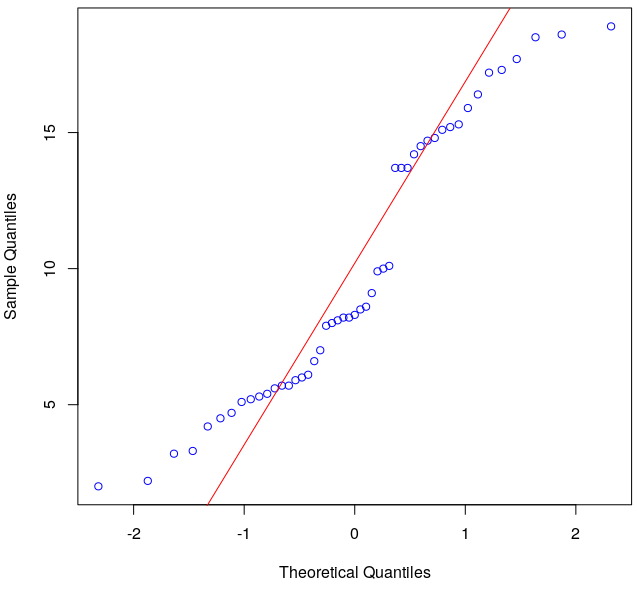
\includegraphics[scale=0.3]{./diagrams/quakes.png}
\end{figure}
\end{frame}

\begin{frame}
  \frametitle{Exercises}
  {\ubung} Listed below are the amounts of mercury (in parts per
  million, or ppm) found in tuna sushi sampled at different stores in
  New York City. The study was sponsored by the New York Times, and
  the stores (in order) are D'Agostino, Eli's Manhattan, Fairway, Food
  Emporium, Gourmet Garage, Grace's Marketplace, and Whole Foods. The
  sample mean is 0.719 ppm and the standard deviation is 0.366 ppm.
  Construct a 90\% confidence interval estimate of the mean amount of
  mercury in the population.

  \begin{alltt}
0.50 0.75 0.10 0.95 1.25 0.54 0.88
  \end{alltt}
\end{frame}

\begin{frame}
  \frametitle{Exercises}
  {\ubung} Here are the numbers of chocolate chips in a sample of 40
  Chips Ahoy regular cookies. The mean is 23.95 chocolate chips and
  the standard deviation is 2.55 chocolate chips. Construct a 99\%
  confidence interval estimate of the mean number of chocolate chips
  in all such cookies. How does the confidence interval not
  contradict the fact that most of the original values do not fall
  between the confidence interval limits?
\end{frame}

\begin{frame}
  \frametitle{Exercises}
  {\ubung} The following data describes a sample of 106 body
  temperatures having a mean of 98.20$^{\circ}$F and a standard
  deviation of 0.62$^{\circ}$F. Construct a 95\% confidence interval
  estimate of the mean body temperature for the entire population.
  What does the result suggest about the common belief that
  98.6$^{\circ}$F is the mean body temperature?
\end{frame}

\begin{frame}
  \frametitle{Body Temperature Data}
  \begin{tabular}{|rrrrrrrrrr|}\hline
    98.6 & 98.6 & 98.0 & 98.0 & 99.0 & 98.4 & 98.4 & 98.4 & 98.4 & 98.6 \\
    98.6 & 98.8 & 98.6 & 97.0 & 97.0 & 98.8 & 97.6 & 97.7 & 98.8 & 98.0 \\
    98.0 & 98.3 & 98.5 & 97.3 & 98.7 & 97.4 & 98.9 & 98.6 & 99.5 & 97.5 \\
    97.3 & 97.6 & 98.2 & 99.6 & 98.7 & 99.4 & 98.2 & 98.0 & 98.6 & 98.6 \\
    97.2 & 98.4 & 98.6 & 98.2 & 98.0 & 97.8 & 98.0 & 98.4 & 98.6 & 98.6 \\
    97.8 & 99.0 & 96.5 & 97.6 & 98.0 & 96.9 & 97.6 & 97.1 & 97.9 & 98.4 \\
    97.3 & 98.0 & 97.5 & 97.6 & 98.2 & 98.5 & 98.8 & 98.7 & 97.8 & 98.0 \\
    97.1 & 97.4 & 99.4 & 98.4 & 98.6 & 98.4 & 98.5 & 98.6 & 98.3 & 98.7 \\
    98.8 & 99.1 & 98.6 & 97.9 & 98.8 & 98.0 & 98.7 & 98.5 & 98.9 & 98.4 \\
    98.6 & 97.1 & 97.9 & 98.8 & 98.7 & 97.6 & 98.2 & 99.2 & 97.8 & 98.0 \\
    98.4 & 97.8 & 98.4 & 97.4 & 98.0 & 97.0 & &&& \\ \hline
  \end{tabular}
\end{frame}

\begin{frame}
  \frametitle{Exercises}
  {\ubung} In a test of weight loss programs, 40 adults used the
  Atkins weight loss program. After 12 months, their mean weight
  loss was found to be 2.1 lb, with a standard deviation of 4.8
  lb. Construct a 90\% confidence interval estimate of the mean
  weight loss for all such subjects. Does the Atkins program
  appear to be effective? Does it appear to be practical?
\end{frame}

% 15. Garlic lor Reducing Cholesterol In a test of the effectiveness of
% garlic for lowering cholesterol, 49 subjects were treated with raw
% garlic. Cholesterol levels were measured before and after the
% treatment. The changes (before minus after) in their levels of LDL
% choies terof (in mg/dL) had a mean of 0,4 and a standatd deviation of
% 21.0 (based on data from “Effect of Raw Garlic VS Commercial Garlic
% Supplements on Flasma I.ipid Concentrations in Adults wiili Moderate
% Hypercholesterolemia,” by Gardner ct al., Archives of Internal
% Medicine, Vol. 167). Construct a 98% confidence interval estimate of
% the mean net change in LDL cholesterol after the garlic treatment-
% What does the confidence interval suggest about the effectiveness of
% garlic in reducing LDL cholesterol?

% 16. Insomnia Treatment A clinical trial was conducted to test the
% effectiveness of the drug zopiclone for treating insomnia in older
% subjects, Before treatment with zopiclone, 16 subjects bad a mean wake
% time of 102.8 min. After treatment with zopiclone, the 16 subjects had
% a mean wake time of 98.9 min and a standard deviation of 42.3 min
% (based on data from “Cognitive Behavioral Therapy vs Zopiclone for
% Treatment of Chronic Primary' Insomnia in Older Adults,” by Siverstcn
% et al., Journal of the American Medical Association, Vol, 295, No.
% 24). Assume that the 16 sample values appear to be from a normally
% distributed population and construct a 98% confidence interval
% estimate of the mean wrake time for a population with zopiclone
% treatments. ’What does the result suggest about the mean wake time of
% 102.8 min before the treatment? Does zopi-clone appear to be
% effective?

% 17. Harry Potter Listed below arc the gross amounts (in millions of
% dollars) earned from box office receipts for the movie Harry Paner and
% the Half-Blood Prince. The movie opened on a Wednesday, and the
% amounts are listed in order for the first 14 days of the movie s
% release. Use the sample values to construct a 99% confidence interval
% estimate of the population mean. What is the population? Identify at
% least one major problem with this data set, 58 22 27 29 21 10 10 8 7 9
% 11 9 4 4

% 18. Years in College Listed below arc the numbers of years it took for
% a random sample of college students to earn bachelor’s degrees (based
% on data from the National Center for Education Statistics). Construct
% a 90% confidence interval estimate of the mean time requited for all
% college students to earn bachelor’s degrees. Docs the confidence
% interval contain the value of 4 years? Is there anything about the
% data that w'ould suggest that the confidence interval might not be a
% good result? 4 4 4 4 4 4 4.5 4.5 4.5 4.5 4,5 4.5 6 6 8 9 9 13 13 15

% 19. Cell Phone Radiation Listed below arc the measured radiation
% emissions (in W/kg) corresponding to these cell phones; Samsung
% SGH-tss9, Blackberry' Storm, Blackberry Curve, Motorola Moto, T-Mobile
% Sidekick, Sanyo Katana Eclipse, Palm Pte, Sony Ericsson, Nokia 6085,
% Apple iPhone 3G S, Kyocera Neo El 100. The data arc from the
% Environmental Working Group. The media often present reports about die
% dangers of cell phone radiation as a cause of cancer. Construct a 90%
% confidence interval estimate of the population mean. What does the
% result suggest about the Federal Communications Commission standard
% that cell phone radiation must be 1.6 W/kg or less?

% 0.38 0.55 1.54 1.55 0.50 0.60 0.92 0.96 1.00 0.86 1.46

% 20. Ages of Race Car Drivons Listed below' arc the ages (years) of
% randomly selected race car drivers (based on data reported in USA
% Today), Construct a 98% confidence interval estimate of the mean age
% of ali race car drivers. 32 32 33 33 41 29 38 32 33 23 27 45 52 29 25

% 21. Lead in Medicine Listed below are die lead concentrations (in
% jUg/g) measured in different Ayurveda medicines. Ayurveda is a
% traditional medical system commonly used in India. The lead
% concentrations listed here are from medicines manufactured in ihe
% United States. The data are based on the article “Lead, Mercury, and
% Arsenic in US and Indian Manufactured Ayurvedic Medicines Sold via the
% Internet,” by Saper et al., journal of the American Medical
% Association, Vol. 300, No. 8. Use the sample data to construct a 95%
% confidence interval estimate of the mean of the lead concentrations
% for the population of all such medicines. If a safety standard
% requires lead concentrations less than 7 /ag/g, does it appear that
% the population mean is less than that level?

% 3.0 6.5 6.0 5.5 20.5 7,5 12,0 20.5 11,5 17.5

% 22. Brain Volume Listed below' arc brain volumes (cm3) of unrelated
% subjects used in a study. (Sec Data Set 6 in Appendix Ë.) Use the
% sample data to construct a 99% confidence interval estimate of the
% mean of the brain volume of the population. Given that typical brain
% volumes ate between 950 cm3 and 1800 cm3, do these values appear to be
% typical? 963 1027 1272 1079 1070 1173 1067 1347 1100 1204 Ages of
% Unsuccessful Applicants 3 477S 4 12344555669 F 3344567 6 0 Ages of
% Successful Applicants 3 367699 4 223344455656677B899 5 1124

% 23. Ays Discrimination? The accompanying stem plots depict ages of
% applicants who were unsuccessful In winning promotion and ages of
% applicants who were successful in winning promotion (based on data
% from “Debating the Use of Statistical Evidence in Allegations of Age
% Discrimination” by Barry and Boland, American Statistician, Vo!. 58,
% No. 2). Assume thaL the samples arc simple random samples and use a
% 95% confidence level to construct the two confidence interval
% estimates of the two population means. Compare the results. What do
% you conclude?

% 24. Intorbraoding of Cultures Changes in head sizes over time suggest
% 	interbreeding with people from other regions. Use the data
% 	depicted in the accompanying dotplots and construct 95%
% 	confidence intervals to determine whether skul! breadths (mm)
% 	appear to have changed from 4000 B.c. to 150 A-D- Explain your
% 	conclusion. .it.:.
	
% 4000 6.C. ISO AD. —i 1 1 1 1 1 - t ■ i ■ t r ■ i ■ i - i rut 120 122
% ]Z4 130 1Z9 ]3tl 13Î 13* ISli 13ft HD 141 Skull Breadth (mm) Sample
% Size, In Exetvitet 25—32, find the sample size required To estimate
% the papulation mean.

\begin{frame}
  \frametitle{Exercises}
  {\ubung} The Wechsler IQ test is designed so that the mean is
  100 and the standard deviation is 15 for the population of
  normal adults. Find the sample size necessary to estimate the
  mean IQ score of professional pilots. We want to be 90\%
  confident that our sample mean is within 3 IQ points of the true
  mean. The mean for this population is clearly greater than 100.
  The standard deviation for this population is probably less than
  15 because it is a group with less variation than a group
  randomly selected from the general population; therefore, if we
  use $\sigma=15$ we are being conservative by using a value that
  will make the sample size at least as large as necessary. Assume
  then that $\sigma=15$ and determine the required sample size.
  Does the sample size appear to be reasonable?
\end{frame}

\begin{frame}
  \frametitle{Exercises}
  {\ubung} As part of a study of grade inflation, you want to
  estimate the mean grade point average of all current college
  students in the United States. All grade point averages are to
  be standardized for a scale between 0 and 4. How many grade
  point averages must be obtained so that the sample mean is
  within $0.2$ of the population mean? Assume that a 99\%
  confidence level is desired. Also assume that a pilot study
  showed that the population standard deviation is estimated to be
  $0.79$. 
\end{frame}

% 27. Buying h Corvette Research of selling prices for used two-year-old
% Corvettes reveals that they have a standard deviation of £2157 (based
% on data from Edmnnds.com). How many selling prices must you obtain in
% order to estimate the mean selling price of these cars? Assume that
% you want 98% confidence that your sample mean is within £250 of the
% population mean. Is it likely that you will find that many
% two-year-old used Gorvettes in your region? ZB. Fficebook Time You
% want to estimate the mean amount of rime Internet users spend on
% Eaccbook each month. How many Internet users must he surveyed in order
% to be 95% confident that your sample mean is within 15 minutes of the
% population mean? Based on results from a prior Nielsen survey, assume
% that the standard deviation of Lhe population of monthly times spent
% on Faccbook is 219 min. What is a ma jot obstacle to getting a good
% estimate of the population mean?

% 29. Sample Size Using Range Rule of Thumb You want to estimate the
% mean SAT score of all college applicants. First use the range rule of
% thumb to make a rough estimate of the standard deviation of those
% scores. Possible SAT scores range from 6ÜÜ to 2400. Use the estimated
% standard deviation to determine the sample size correspond Eng to a
% 98% confidence level and a margin of error of I 00 points. What isn’t
% quite right with this exercise?

% 30. Sample Size Using Range Rule of Thumb You want to estimate the
% mean amount of annual tuition being paid by current full-time college
% students in the United States. First use the range role ot thumb to
% make a rough estimate of the standard deviation of the amounts spent-
% It is reasonable to assume that tuition amounts range from £0 to about
% £45, 000. Then use that estimated standard deviation to determine rht
% sample size corresponding to 99% confidence and a £100 margin of
% error. Does the resulting sample size seem practical?

% 31. Sample Size Using Sample Data Refer to Data Set 1 in Appendix B
% and find the maximum and minimum pulse lates for males, then use those
% values with the range rule of thumb to estimate cr How many adult
% males must you randomly select and test if you want to be 95%
% confident that the sample mean pulse rate is within 2 beats (per
% minute) of the true population mean ju. The standard deviation of the
% 40 puise ta tes of males in Data Set 1 is 10.3 beats per minute. If,
% instead of using the range rule of thumb, the standard deviation of
% the sample is used as an estimate of cr, is the required sample size
% very different? Which result is likely to be closer to the correct
% sample size?

% 32. Sample Size Using Sample Data Refer to Data Sel 16 in Appendix B
% and find the maximum and minimum earthquake magnitudes, then use those
% values with the range rule of thumb to estimate cr. How many
% earthquakes must you randomly select if you want to be 95% confident
% that the sample mean magnitude is within 0.2 of the true population
% mean ft! The standard deviation of the 50 earthquake magnitudes in
% Data Set 16 is 0. 587. Find the required sample siie by using the
% standard deviation of tire sample as an estimate ofrr. Which of the
% two results is likely to he better? Appendix B Data Sets. In Exercises
% 33 and 34, use the data sets from Appendix B,

% 33. Earthquake Magnitudes Lise the earthquake magnitudes listed in
% Data Set 16 from Appendix B and construct a 99% confidence interval
% estimate of the mean of all such magnitudes.

% 34. Second-Hand Smoke Figure 7-6 from Example 5 shows a graph of throe
% different confidence intervals. Use the cotitune levels of smokers
% listed in Data Set 9 from Appendix B and construct the 95% confidence
% interval estimate of rite population mean p.

\begin{frame}
  \frametitle{Term Test B Question 1}
A production cycle requires good weather. In September,
based on many years of experience, {\puw} out of {\iex} days have good enough
weather for the production cycle. Calculate the probability that
on exactly four out of these five days the weather was good enough for
the production cycle:

\begin{tabular}{l}
  September 5, 2011 \\
  September 5, 2012 \\
  September 5, 2013 \\
  September 5, 2014 \\
  September 5, 2015 \\
\end{tabular}
\end{frame}

\begin{frame}
  \frametitle{Term Test B Question 2}
  In a meat manufacturing plant, {\nae} cattle are processed per
hour at a work station. {\mih}\% of the processed cattle create problems
that cause an interruption in the work flow. Calculate the probability
that a work station will experience strictly less than four
interruptions on a given work day (eight hours). 
\end{frame}

\begin{frame}
  \frametitle{Term Test B Question 3}
  A factory worker produces a mean of {\esh} units of a food
product per hour with a standard deviation of {\chu} units. The
distribution is normal. What is the probability that the worker
produces more than {\pee} units in a day (where one work day has eight
hours). Assume that hourly outputs on a given day are independent of
each other (unlikely in real life). Hint: Treat the production per day
as a sample of eight hourly outputs and use the Central Limit Theorem.
\end{frame}

\begin{frame}
  \frametitle{Term Test B Question 4}
  A company that makes processed foods receives an
ingredient in single units from a supplier. {\ood}\% of the ingredients
are A-grade quality, {\tee}\% are B-grade quality, and the rest is
spoiled. On Tuesday, the supplier drops off {\aih} units. Estimate the
probability that {\aoj} or more units are spoiled.
\end{frame}

\begin{frame}
  \frametitle{Term Test B Question 5}
  A bakery product maintains its quality for a mean of {\eep}
hours after production with a standard deviation of {\eim} hours. The
distribution is normal. The ``best before'' date is chosen such that
{\sho}\% of the product maintain their quality by that date. How many
hours after production should the ``best before'' date be set?
\end{frame}

\begin{frame}
  \frametitle{Estimating a Population Variance}
  \begin{description}
  \item[Point Estimate] The sample variance $s^{2}$ is the best point
    estimate of the population variance $\sigma^{2}$. The sample
    standard deviation $s$ is commonly used as a point estimate of
    $\sigma$ even though it is a biased estimator.
  \item[Confidence Interval] When constructing a confidence interval
    estimate of a population standard deviation or population
    variance, we construct the confidence interval using the
    \alert{$\chi^{2}$ (chi-square) distribution}.
  \end{description}
\end{frame}

\begin{frame}
  \frametitle{Chi-Square Distribution}
The sample statistic
\begin{equation}
  \label{eq:neechooy}
  \chi^{2}=\frac{(n-1)s^{2}}{\sigma^{2}}
\end{equation}
has a sampling distribution called the chi-square distribution. The
chi-square distribution is skewed, so the right tail and the left tail
are not symmetrical. We call the critical value for the right tail
$\chi_{R}^{2}$ and the critical value for the left tail
$\chi_{L}^{2}$.
\begin{figure}[h]
  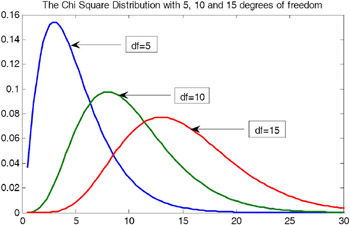
\includegraphics[scale=0.5]{./diagrams/chisqu.jpg}
\end{figure}
\end{frame}

\begin{frame}
  \frametitle{Confidence Interval for Population Variance}
  \begin{description}
  \item[Objective] Construct a confidence interval used to estimate a
    population standard deviation or variance
  \item[Notation] $\sigma$ is the population standard deviation;
    $\sigma^{2}$ is the population variance; $s$ is the sample
    standard deviation; $s^{2}$ is the sample variance; $n$ is the
    sample size; and $E$ is the margin of error
  \item[Required] A simple random sample and a normally distributed
    population even if the sample is large!
  \end{description}
\end{frame}

\begin{frame}
  \frametitle{Confidence Interval for Population Variance}
  \begin{block}{confidence interval for population variance}
    \begin{equation}
      \label{eq:zaozienu}
      \frac{(n-1)s^{2}}{\chi_{R}^{2}}<\sigma^{2}<\frac{(n-1)s^{2}}{\chi_{L}^{2}}
    \end{equation}
  \end{block}

\medskip

  \begin{block}{confidence interval for population standard deviation}
    \begin{equation}
      \label{eq:eikogohg}
      \sqrt{\frac{(n-1)s^{2}}{\chi_{R}^{2}}}<\sigma<\sqrt{\frac{(n-1)s^{2}}{\chi_{L}^{2}}}\notag
    \end{equation}
  \end{block}
with $df=n-1$.
\end{frame}

\begin{frame}
  \frametitle{Exercises}
  {\ubung} The following data describes a sample of 106 body
  temperatures having a mean of 98.20$^{\circ}$F and a standard
  deviation of 0.62$^{\circ}$F. Construct a 90\% confidence interval
  estimate of the standard deviation of the body temperature for the
  entire population. 
\end{frame}

\begin{frame}
  \frametitle{Body Temperature Data}
  \begin{tabular}{|rrrrrrrrrr|}\hline
    98.6 & 98.6 & 98.0 & 98.0 & 99.0 & 98.4 & 98.4 & 98.4 & 98.4 & 98.6 \\
    98.6 & 98.8 & 98.6 & 97.0 & 97.0 & 98.8 & 97.6 & 97.7 & 98.8 & 98.0 \\
    98.0 & 98.3 & 98.5 & 97.3 & 98.7 & 97.4 & 98.9 & 98.6 & 99.5 & 97.5 \\
    97.3 & 97.6 & 98.2 & 99.6 & 98.7 & 99.4 & 98.2 & 98.0 & 98.6 & 98.6 \\
    97.2 & 98.4 & 98.6 & 98.2 & 98.0 & 97.8 & 98.0 & 98.4 & 98.6 & 98.6 \\
    97.8 & 99.0 & 96.5 & 97.6 & 98.0 & 96.9 & 97.6 & 97.1 & 97.9 & 98.4 \\
    97.3 & 98.0 & 97.5 & 97.6 & 98.2 & 98.5 & 98.8 & 98.7 & 97.8 & 98.0 \\
    97.1 & 97.4 & 99.4 & 98.4 & 98.6 & 98.4 & 98.5 & 98.6 & 98.3 & 98.7 \\
    98.8 & 99.1 & 98.6 & 97.9 & 98.8 & 98.0 & 98.7 & 98.5 & 98.9 & 98.4 \\
    98.6 & 97.1 & 97.9 & 98.8 & 98.7 & 97.6 & 98.2 & 99.2 & 97.8 & 98.0 \\
    98.4 & 97.8 & 98.4 & 97.4 & 98.0 & 97.0 & &&& \\ \hline
  \end{tabular}
\end{frame}

\begin{frame}
  \frametitle{Exercises}
  {\ubung} A container of car antifreeze is supposed to hold 3785 mL
  of the liquid. Realizing that fluctuations are inevitable, the
  quality control manager wants to be sure that the standard deviation
  is less than 30 mL. Otherwise, some containers would overflow while
  others would not have enough of the coolant. She selects a simple
  random sample of 24 containers and finds that the mean is 3789 mL
  and the standard deviation is 42.8 mL. Use these sample results to
  construct the 99\% confidence interval for the true value of
  $\sigma$. Does this confidence level suggest that the variation is
  at an acceptable level?
\end{frame}

\begin{frame}
  \frametitle{Exercises}
  {\ubung} Use the following data set (next slide) of the weight of
  post-1983 pennies to construct a 98\% confidence interval estimate
  of the standard deviation of the weights of all post-1983 pennies.
  Assume that the weights are normally distributed. The sample mean is
  $\bar{x}=2.4988$, the sample standard deviation is $s=0.016636$.
\end{frame}

\begin{frame}
  \frametitle{Exercises}
  \begin{tabular}{|rrrrrr|}\hline
2.5113 & 2.4907 & 2.5024 & 2.5298 & 2.4950 & 2.5127 \\
2.4998 & 2.4848 & 2.4823 & 2.5163 & 2.5222 & 2.5004 \\
2.5248 & 2.5058 & 2.4900 & 2.5068 & 2.5016 & 2.4797 \\
2.5067 & 2.5139 & 2.4762 & 2.5004 & 2.5170 & 2.4925 \\
2.4876 & 2.4933 & 2.4806 & 2.4907 & 2.5017 & 2.4950 \\
2.4973 & 2.5252 & 2.4978 & 2.5073 & 2.4658 & 2.4529 \\ \hline
  \end{tabular}
\end{frame}

\begin{frame}
  \frametitle{One Sample Flow Chart}
  \begin{figure}[h]
    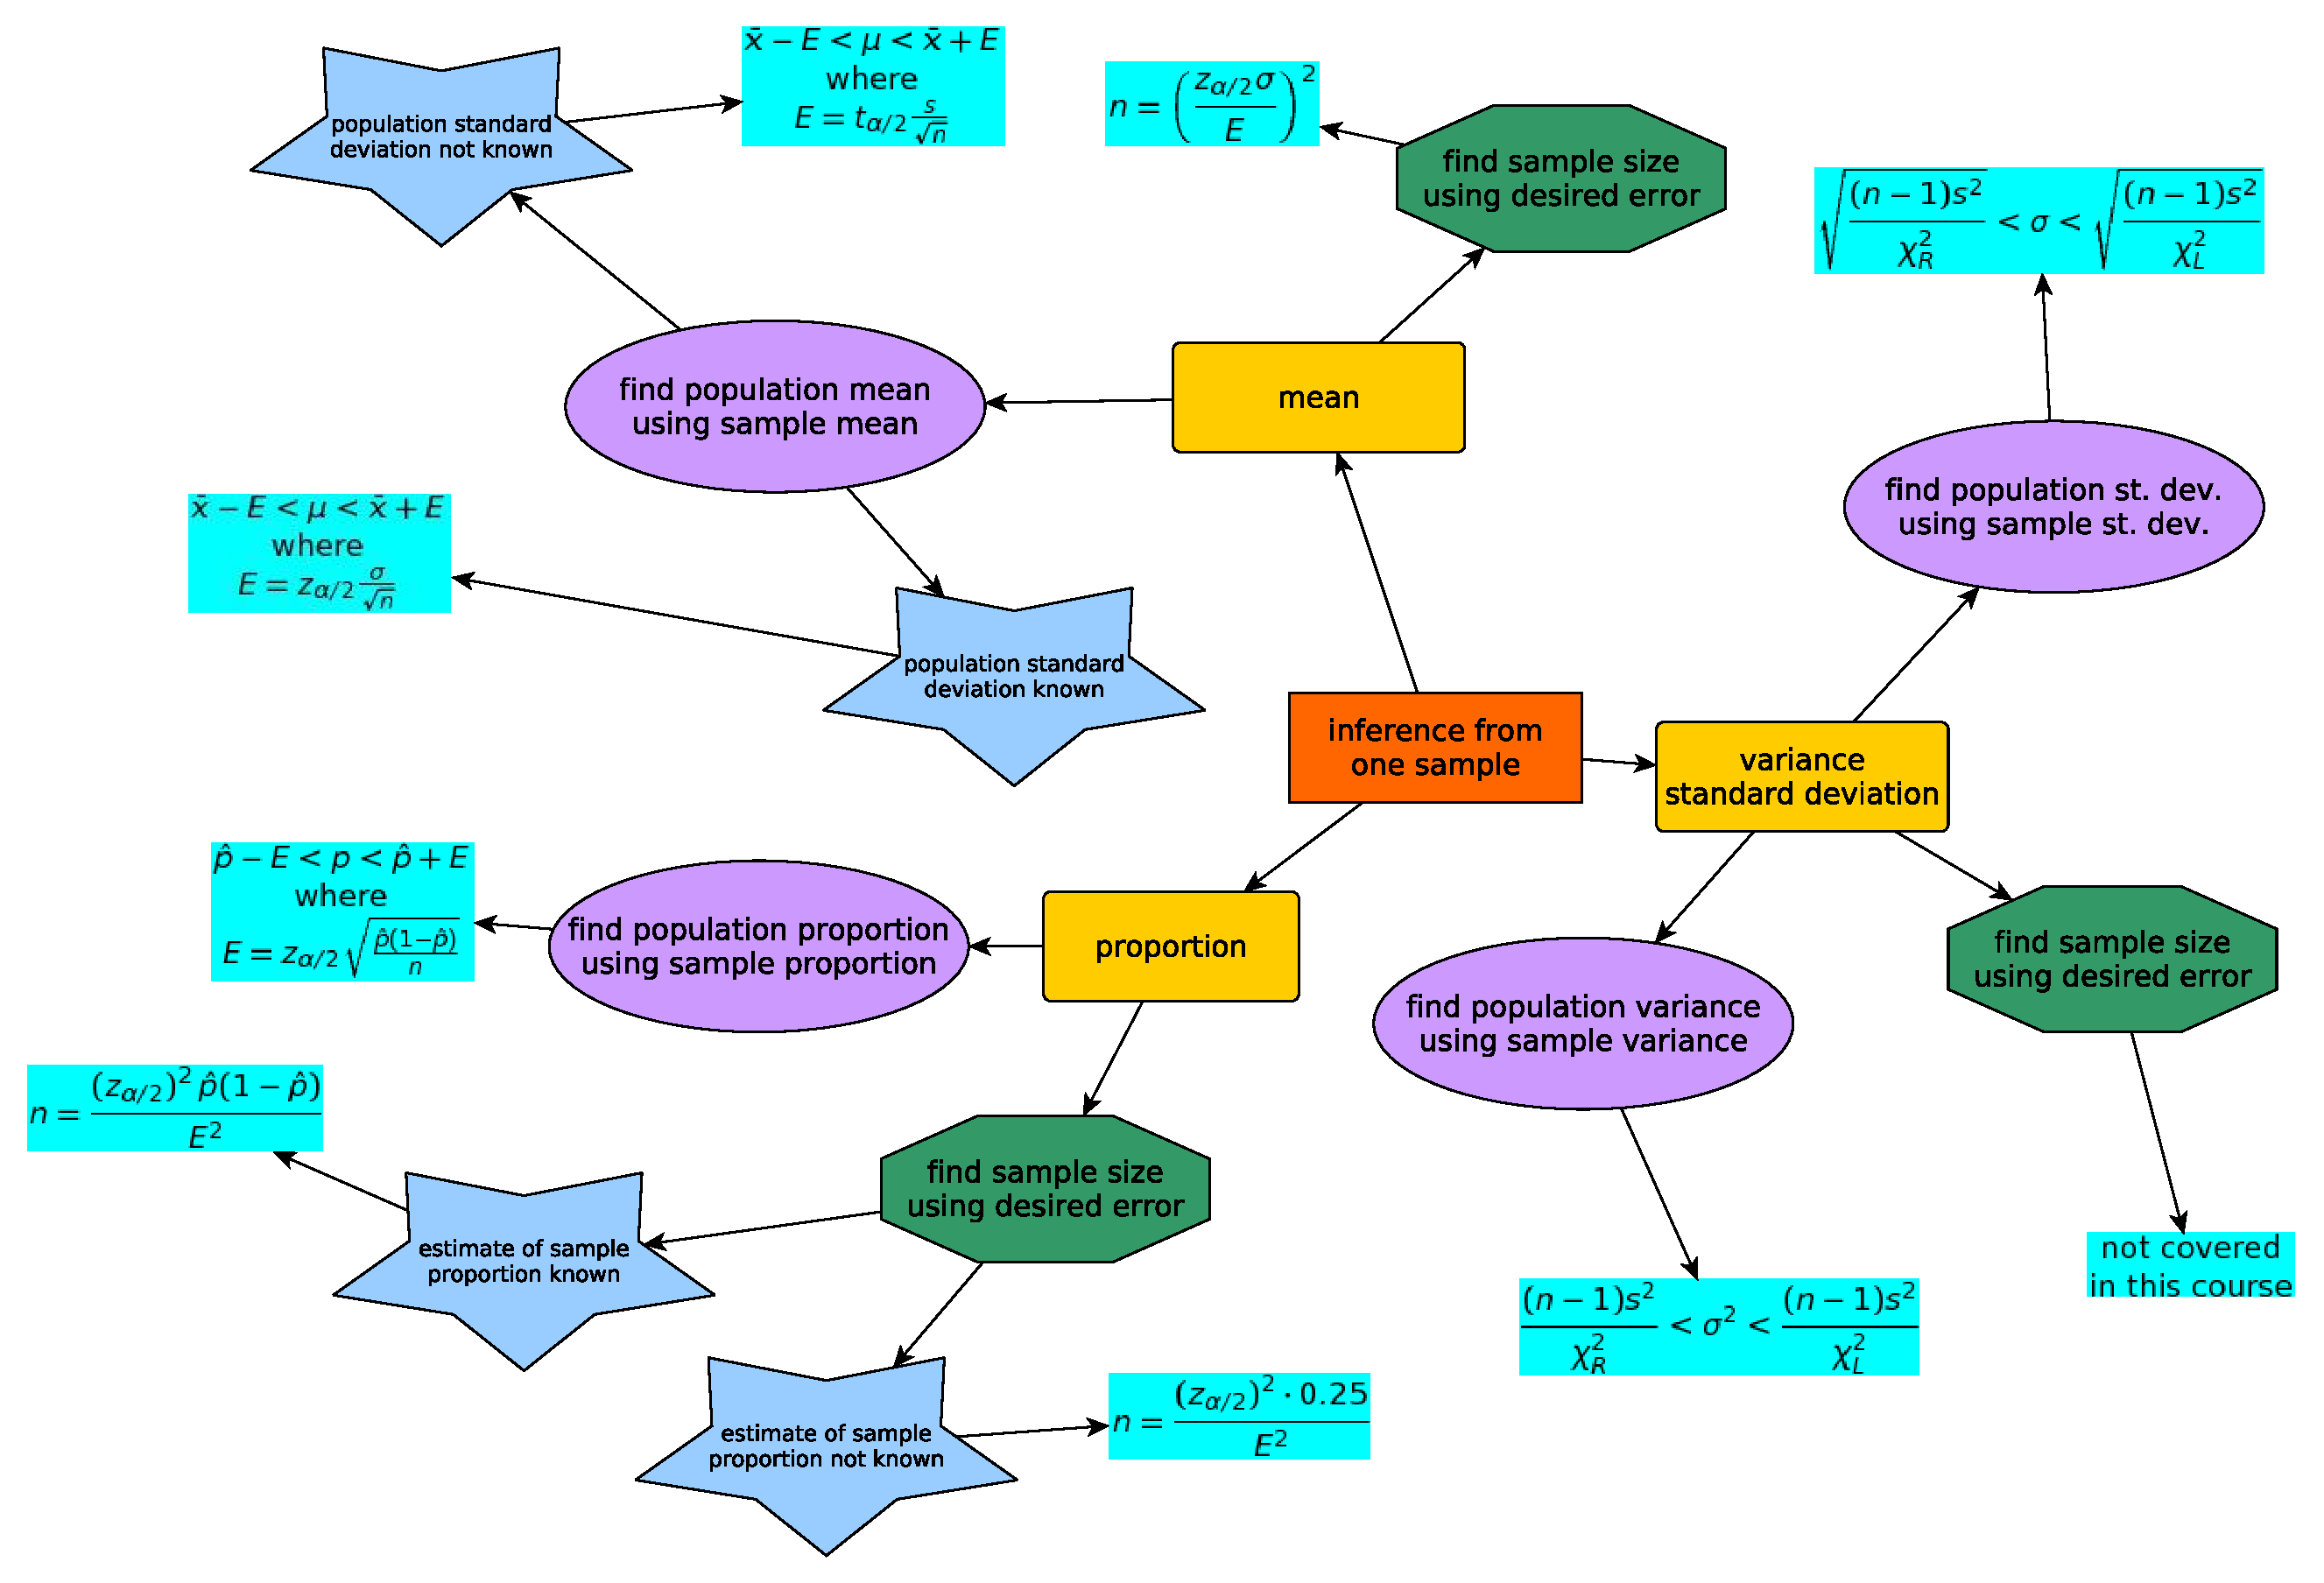
\includegraphics[scale=0.255]{./diagrams/onesample.pdf}
  \end{figure}
\end{frame}

\begin{frame}
  \frametitle{End of Lesson}
Next Lesson: Hypothesis Testing 
% I am changing the schedule to align with Triola, HT before 2pop
\end{frame}

\end{document}
